%%%%%%%%%%%%%%%%%%%%%%%%%%%%%%%%%%%%%%%%%%%%%%%%%%%%%%%%%%%%%%%%%%%%%%%%%%%
%% This file is part of the book
%%
%% Algorithmic Graph Theory
%% http://code.google.com/p/graph-theory-algorithms-book/
%%
%% Copyright (C) 2009--2011 Minh Van Nguyen <nguyenminh2@gmail.com>
%%
%% See the file COPYING for copying conditions.
%%%%%%%%%%%%%%%%%%%%%%%%%%%%%%%%%%%%%%%%%%%%%%%%%%%%%%%%%%%%%%%%%%%%%%%%%%%

\documentclass{article}

\usepackage{tikz}
\usetikzlibrary{external}
\tikzexternalize{determine-eccentricity-radius-diameter}

\begin{document}

\begin{figure}
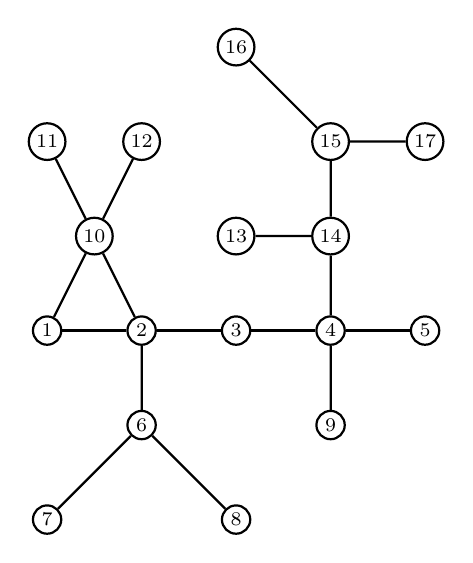
\begin{tikzpicture}
[lineDecorate/.style={-,thick},%
  nodeDecorate/.style={shape=circle,inner sep=1.5pt,draw,thick},%
  scale=1.2]
\scriptsize
%% nodes or vertices
\foreach \nodename/\x/\y in {
  1/1/0, 2/2/0, 3/3/0, 4/4/0, 5/5/0, 6/2/-1, 7/1/-2, 8/3/-2, 9/4/-1,
  10/1.5/1, 11/1/2, 12/2/2, 13/3/1, 14/4/1, 15/4/2, 16/3/3, 17/5/2}
{
  \node (\nodename) at (\x,\y) [nodeDecorate] {$\nodename$};
}
%% edges or lines
\path
\foreach \startnode/\endnode in {
  1/2, 1/10, 2/3, 2/6, 2/10, 3/4, 4/5, 4/9, 4/14, 6/7, 6/8, 10/11,
  10/12, 13/14, 14/15, 15/16, 15/17}
{
  (\startnode) edge[lineDecorate] node {} (\endnode)
};
\end{tikzpicture}
\end{figure}

\end{document}
